\section{1174050 Dika Sukma Pradana}

\subsection{Teori}
\begin{enumerate}
\item Jelaskan apa itu klasifikasi teks, sertakan gambar ilustrasi buatan sendiri.\par
Klasifikasi teks adalah proses pemberian tag atau kategori ke teks sesuai dengan isinya. Ini salah satu tugas mendasar dalam Natural Language Processing (NLP) dengan aplikasi luas seperti analisis sentimen, pelabelan topik, deteksi spam, dan deteksi maksud.

\begin{figure}[ht]
\centering
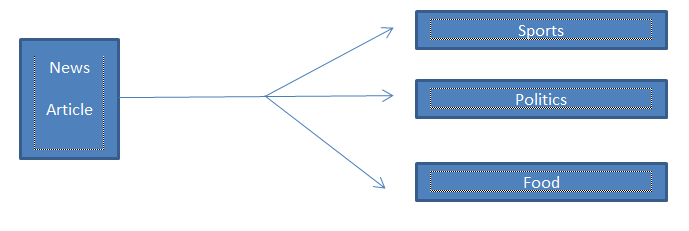
\includegraphics[scale=0.2]{figures/1174050/chapter4/1.PNG}
\caption{contoh klasifikasi teks}
\label{contoh}
\end{figure}

\item Jelaskan mengapa klasifikasi bunga tidak bisa menggunakan machine learning, sertakan ilustrasi sendiri.\par
Dikarenakan tidak semua bunga memliki ciri - ciri yang sama. Atau dalam kata lain terdapat data noise dalam klasifikasi bunga sehingga tidak bisa menggunakan machine learning.\\
Contohnya Anggrek memiliki warna ungu, dengan jumlah kelopak 5. Kemudian ada bunga warna ungu dengan jumlah kelopak yang sama namun ternyata bukan anggrek dan kategorinya banyak sekali. Bahkan ada bunga yang tidak jelas apakah warnanya sesuai atau tidak, sehingga bisa menyebabkan data noise. 

\begin{figure}[ht]
\centering
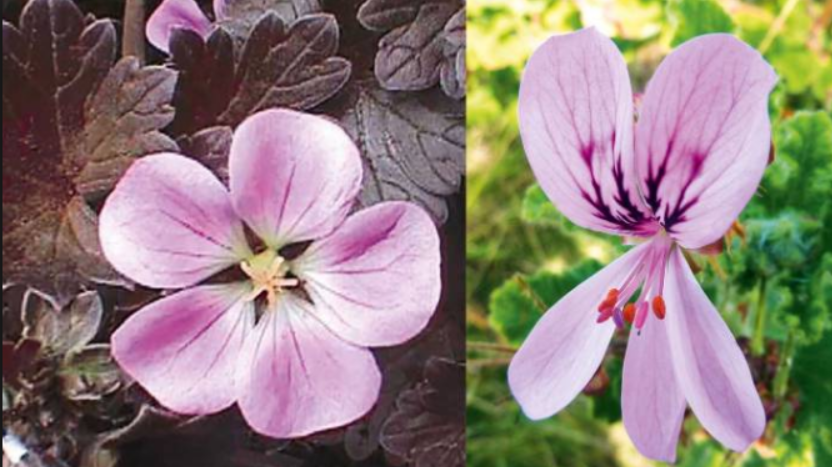
\includegraphics[scale=0.2]{figures/1174050/chapter4/2.PNG}
\caption{contoh klasifikasi bunga}
\label{contoh}
\end{figure}

\item Jelaskan bagaimana teknik pembelajaran mesin pada teks pada kata-kata yang digunakan di youtube,jelaskan arti per atribut data csv dan sertakan ilustrasi buatan sendiri.\par
Youtube akan mengingat kata - kata yang sering kira gunakan pada bagian search. seperti pada saat kita menginputkan huruf r maka akan muncul rekomendasi dari youtube baik yang sudah pernah kita cari atau yang belum pernah.

\begin{figure}[ht]
\centering
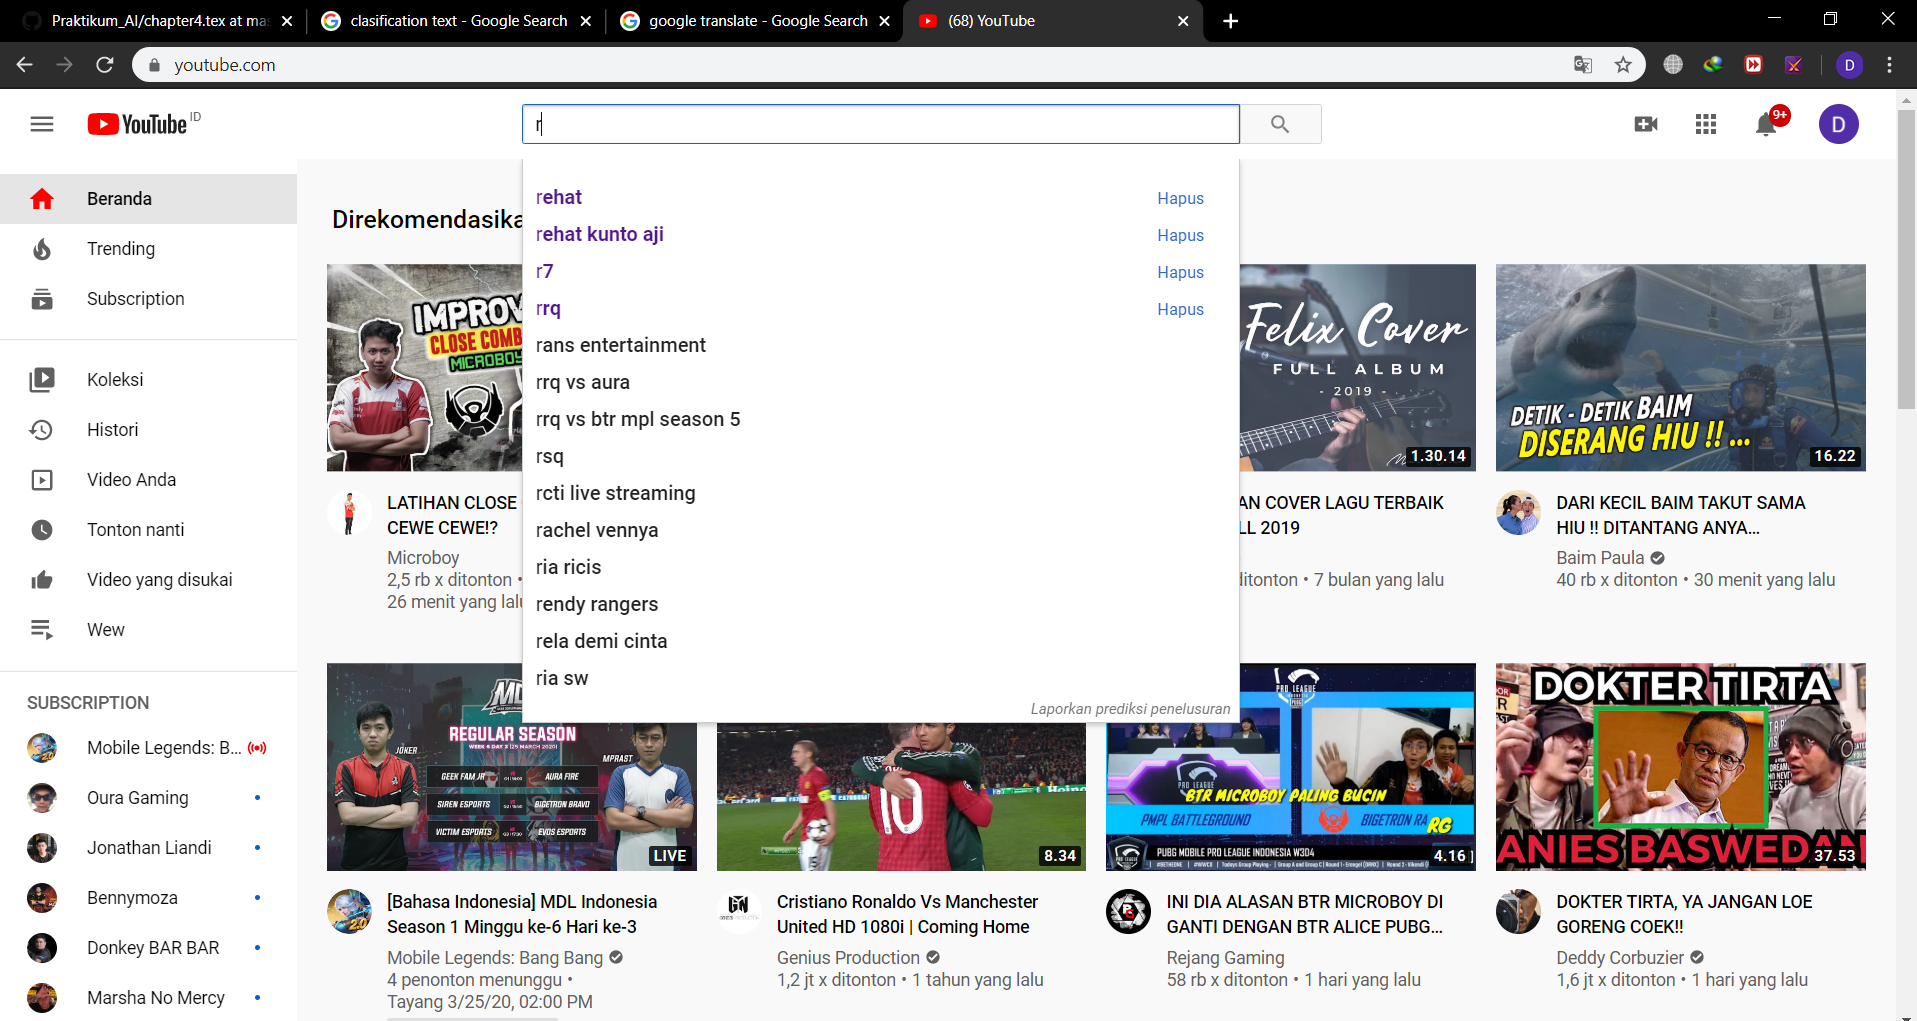
\includegraphics[scale=0.2]{figures/1174050/chapter4/3.PNG}
\caption{contoh teknik pembelajaran mesin}
\label{contoh}
\end{figure}

\item Jelaskan apa yang dimaksud vektorisasi data.\par
Pembagian dan pemecahan data, kemudian dilakukan perhitungan. Vektorisasi juga dapat dimaksudkan dengan setiap data yang mungkin dipetakan ke integer tertentu. jika kita memiliki array yang cukup besar maka setiap kata / data cocok dengan slot unik dalam array (nilai pada indeks adalah nomor satu kali kata itu muncul).

\item Jelaskan apa itu bag of words dengan kata-kata yang sederhana dan ilustrasi sendiri.
 Bag-of-words ialah sebuah gambaran sederhana digunakan dalam pengolahan bahasa alami dan pencarian informasi. Dikenal sebagai model ruang vektor. Pada model ini, tiap kalimat dalam dokumen digambarkan sebagai token, mengabaikan tata bahasa dan bahkan urutan kata namun menghitung frekuensi kejadian atau kemunculan kata dari dokumen.
 
\begin{figure}[ht]
\centering
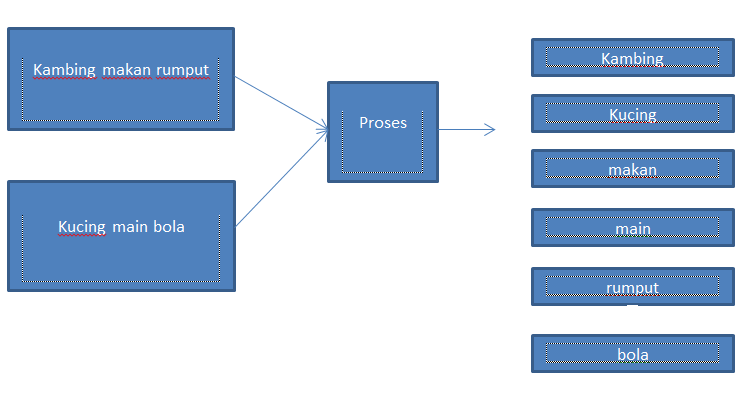
\includegraphics[scale=0.2]{figures/1174050/chapter4/4.PNG}
\caption{contoh bag of words}
\label{contoh}
\end{figure}

\item Jelaskan apa itu TF-IDF, ilustrasikan dengan gambar sendiri.
TF-IDF  memberi kita frekuensi kata dalam setiap dokumen dalam korpus atau mengganti data jadi number. Ini adalah rasio berapa kali kata itu muncul dalam dokumen dibandingkan dengan jumlah total kata dalam dokumen itu. Itu meningkat seiring jumlah kemunculan kata itu di dalam dokumen meningkat. Setiap dokumen memiliki tf sendiri.
 
\begin{figure}[ht]
\centering
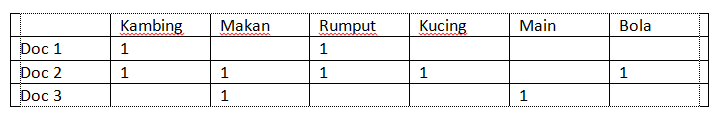
\includegraphics[scale=0.2]{figures/1174050/chapter4/5.PNG}
\caption{contoh TF-IDF}
\label{contoh}
\end{figure}

\end{enumerate}


\subsection{Praktek Program}
\begin{enumerate}
\item import data pandas dan 500 baris data dummy kemudian di jelaskan tiap barisnya.
\lstinputlisting{src/1174050/chapter4/1.py}
\begin{figure}[ht]
\centering
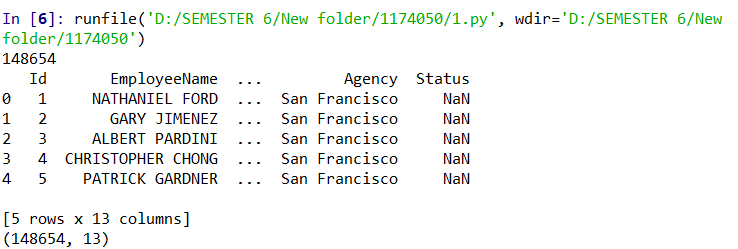
\includegraphics[scale=0.5]{figures/1174050/chapter4/6.PNG}
\caption{hasil}
\label{Praktek no 1}
\end{figure}

\item memecah data prame menjadi dua yag pertama 450 dan kedua sisanya 50
\lstinputlisting{src/1174050/chapter4/2.py}
\begin{figure}[ht]
\centering
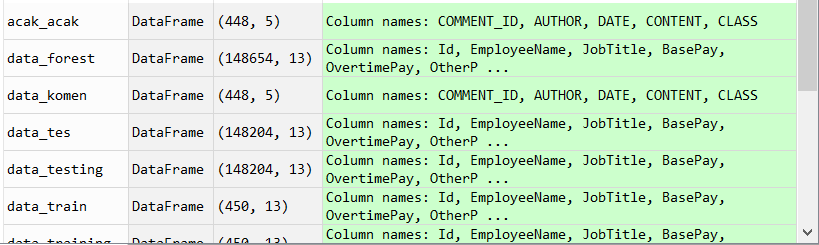
\includegraphics[scale=0.5]{figures/1174050/chapter4/7.PNG}
\caption{hasil}
\label{Praktek no 2}
\end{figure}

\item praktek vektorisasi\par
berikut merupakan codingan untuk melakukan vektorisasi data berupa teks dalam format csv
\lstinputlisting{src/1174050/chapter4/3.py}
\begin{figure}[ht]
\centering
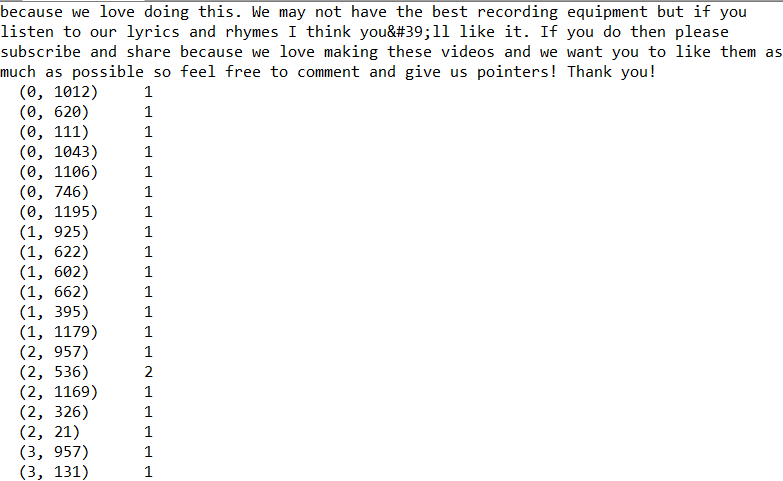
\includegraphics[scale=0.5]{figures/1174050/chapter4/8.PNG}
\caption{hasil}
\label{Praktek no 3}
\end{figure}
 import library pandas yang di inisialisasi menjadi pd setelah itu ada dibuat class dan method untuk membaca file csv yang di masukan alamatnya pada kurung, lakukan klasifikasi samadengan 1 merupakan spam dan class samadengan 0 bukan spam setelah itu masukan librari CountVektorizer yang digunakan untuk vektorisasi data, lalu dilanjutkan pada bagian dibuat variabel yang berisi vektorisasi dari data di field content setelah itu variabel tersebut di running hasilnya menunjukan 350 baris di kali 1738 kolom selanjutnya dicoba untuk memunculkan isi recod pada baris ke 349 maka akan muncul isian dari baris tersebut. selanjutnya dibuat variabel yang berisi data hasil vektorisasi setelah yang terdiri dari variabel yang berisi data komen yang di dalamnya di buat random yang nantinya akan dibut data training dan data testing dengan ketentuan data training 300 dan data testing sebanyak 50 setelah itu data training di lakukan vektorisasi dan data testing juga dilakukan vektorisasi setelah itu kedua data training dan testing tersebut dibuat label dengan parameter field CLASS.

\item klasifikasi SVM
 berikut kodingnya :
\lstinputlisting{src/1174050/chapter4/4.py}
\begin{figure}[ht]
\centering
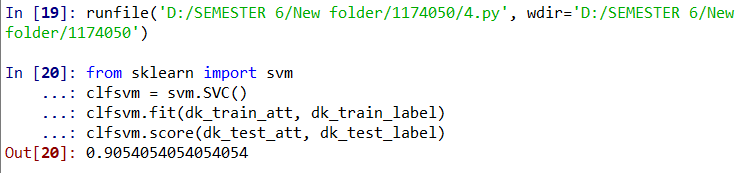
\includegraphics[scale=0.5]{figures/1174050/chapter4/9.PNG}
\caption{hasil}
\label{Praktek no 4}
\end{figure}
melakukan verifikasi import librari svm dari sklearn kemudian membuat variabel clfsvm berisikan method svc setelah itu variabel tersebut di berikan method fit dengan isian data train vektorisasi dan data training label yang berguna untuk melatih data tersebut setelah itu di coba untuk memunculkan score atau akurasi dari data tersebut menggunakan data testing vektorisasi dan data testing label.

\item klasifikasi decision tree 
berikut ini merupakan codingan klasifikasi decision tree
\lstinputlisting{src/1174050/chapter4/5.py}
\begin{figure}[ht]
\centering
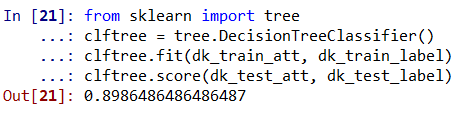
\includegraphics[scale=0.5]{figures/1174050/chapter4/10.PNG}
\caption{hasil}
\label{Praktek no 5}
\end{figure}
import library tree dari sklearn kemudian membuat variabel clftree berisikan method DecisionTreeClasifier setelah itu variabel tersebut di berikan method fit dengan isian data train vektorisasi dan data training label yang berguna untuk melatih data tersebut agar dapat digunakan pada codingan selanjutnya setelah itu di coba untuk memunculkan score atau akurasi dari data tersebut menggunakan data testing vektorisasi dan data testing label.

\item plot comfusion matrix
berikut merupakan codingan untuk confusion matrix 
\lstinputlisting{src/1174050/chapter4/6.py}
\begin{figure}[ht]
\centering
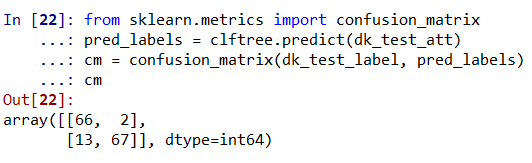
\includegraphics[scale=0.5]{figures/1174050/chapter4/11.PNG}
\caption{hasil}
\label{Praktek no 6}
\end{figure}
import library comfusion matrix selanjutnya dilakukan prediksi pada pada data tes nya kemudian data tersebut di masukan kedalam variabel cm dengan method confusion matrix yang di dalamnya terdapat data dari variabel perd label dan dk test label setelah itu variabel cm tersebut di running maka akan memunculkan nilai matrixnya. 

\item cross valodation 
berikut merupakan code untuk cross validation pada codingan pertama yaitu melakukan split 5 kali yaoti mengitung tingkat akurasi menggunakan data training.
\lstinputlisting{src/1174050/chapter4/7.py}
\begin{figure}[ht]
\centering
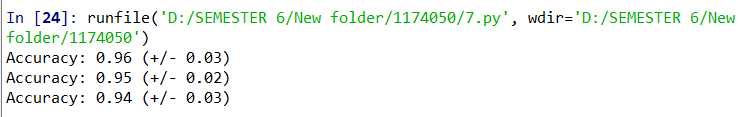
\includegraphics[scale=0.5]{figures/1174050/chapter4/12.PNG}
\caption{hasil}
\label{Praktek no 7}
\end{figure}
akan di bandingkan tingkat akurasi dari semua hasil akurasiya yang akan memunculkan nilai akurasi dari tiga metode yaitu random forest, decision tree, dan klasifikasi svm (suport vector machine) diamana mana yang terbaik dan lebih akurat pada hasilnya data yang paling akurat yaitu random forest. terdapat grafik data yang terdapat dari grafik tersebut di dapat dari codingan dengan cara pengulangan data masing masing 10 kali setelah itu di eksekusi menjadi grafik berbentuk 3D pada gambar tersebut menunjukan rasio dari yang terrendah yaitu data SVM kemudian data decision tree dan hasil random forest.


\item Pengamatan program 
\lstinputlisting{src/1174050/chapter4/8.py}
\begin{figure}[ht]
\centering
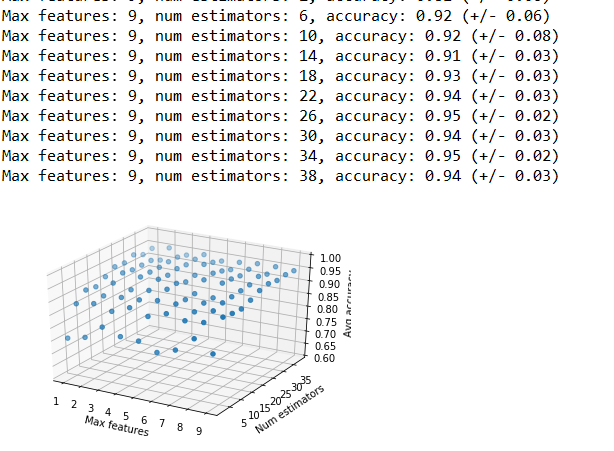
\includegraphics[scale=0.5]{figures/1174050/chapter4/13.PNG}
\caption{hasil}
\label{Praktek no 8}
\end{figure}
\end{enumerate}


\subsection{Penanganan Error}
\begin{enumerate}
\item screenshoot error

\begin{figure}[ht]
\centering
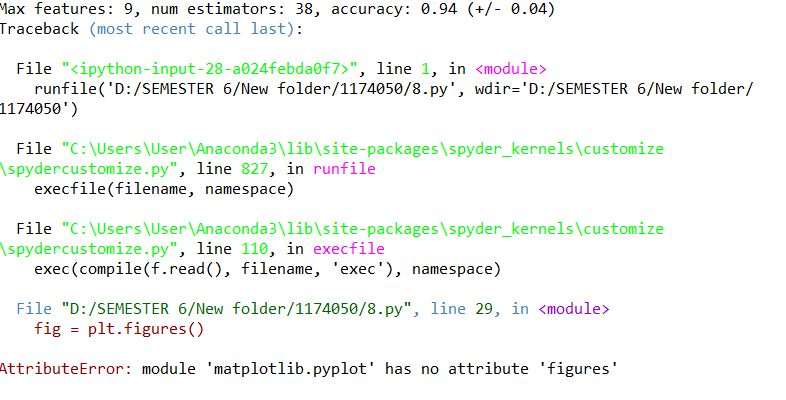
\includegraphics[scale=0.5]{figures/1174050/chapter4/error.PNG}
\caption{hasil}
\label{Error}
\end{figure}

\item codingan yang error 
\begin{verbatim}
# -*- coding: utf-8 -*-
"""
Created on Mon Mar 23 22:19:22 2020

@author: User
"""

from sklearn.ensemble import RandomForestClassifier
import numpy as np
max_features_opts = range(1, 10, 1)
n_estimators_opts = range(2, 40, 4)
rf_params = np.empty((len(max_features_opts)*len(n_estimators_opts),4), float)
i = 0
for max_features in max_features_opts:
    for n_estimators in n_estimators_opts:
        clf = RandomForestClassifier(max_features=max_features,n_estimators=n_estimators)
        scores = cross_val_score(clf, dk_train_att, dk_train_label, cv=5)
        rf_params[i,0] = max_features
        rf_params[i,1] = n_estimators
        rf_params[i,2] = scores.mean()
        rf_params[i,3] = scores.std() * 2
        i += 1
        print("Max features: %d, num estimators: %d, accuracy: %0.2f (+/- %0.2f)" 
%   (max_features, n_estimators, scores.mean(), scores.std() * 2))
        
import matplotlib.pyplot as plt
from mpl_toolkits.mplot3d import Axes3D
from matplotlib import cm
fig = plt.figures()
fig.clf()
ax = fig.gca(projection='3d')
x = rf_params[:,0]
y = rf_params[:,1]
z = rf_params[:,2]
ax.scatter(x, y, z)
ax.set_zlim(0.6, 1)
ax.set_xlabel('Max features')
ax.set_ylabel('Num estimators')
ax.set_zlabel('Avg accuracy')
plt.show()
\end{verbatim}
\item solusinya
Didalam library matplotlib tidak ada attribute figures tetapi figure makanya pada koding diatas error karena menggunakan figures yang harusnya menggunakan figure.
\end{enumerate}